\documentclass[10pt]{article}

\usepackage[utf8]{inputenc}
\usepackage[spanish]{babel}

\usepackage{hyperref}

\usepackage{graphicx}
\graphicspath{ {images/} }


\usepackage{fancyhdr} % Headers and footers
\pagestyle{fancy} % All pages have headers and footers
\fancyhead{} % Blank out the default header
\fancyfoot{} % Blank out the default footer
\fancyhead[C]{ \today \ $\bullet$ Profesión y Sociedad $\bullet$ Licencias Software } % Custom header text
\fancyfoot[RO] {\thepage}



\begin{document}

%----------------------------------------------------------------------------------------
%	TITLE SECTION
%----------------------------------------------------------------------------------------
	\begin{titlepage}
      \centering
          %\includegraphics[width=0.15\textwidth]{example-image-1x1}\par\vspace{1cm}
          {\scshape\LARGE Universidad de Valladolid \par}
          \vspace{1cm}
          {\scshape\Large Profesión y Sociedad.\par}
          \vspace{1.5cm}
          {\huge\bfseries Licencias Software \par}
          \vspace{2cm}
          {\large
          \textsc{Amigo Alonso, Alberto}\\[2mm] % Your name
          \textsc{Delgado Álvarez, Sergio}\\[2mm] % Your name
          \textsc{García Prado, Sergio}\\[2mm] % Your name
          \textsc{Iglesias Cortijo, David}\\[2mm] % Your name

          \vspace{-5mm}
          }

          \vfill
		% Bottom of the page
		{\large \today\par}
	\end{titlepage}

%----------------------------------------------------------------------------------------
%	TABLE OF CONTENTS
%----------------------------------------------------------------------------------------

	\clearpage
	\tableofcontents

%----------------------------------------------------------------------------------------
%	TEXT
%----------------------------------------------------------------------------------------

	\clearpage
    \section{Introducción}		
        \paragraph{}
        Hoy en día, en el seno de una revolución tecnológica de más de cincuenta años, no es concebible el avance de la civilización sin los componentes electrónicos que acompañan a cada individuo. El conjunto de estos componentes está formado por una gran variedad de ensamblajes: desde dispositivos móviles que son usados en cada instante, pasando por sistemas empotrados que controlan la producción y movilidad en tiempo real, hasta supercomputadores especializados en el cálculo científico.
        
        \paragraph{}
        Todos estos dispositivos tienen en común que, a pesar de poseer diferentes configuraciones de hardware para ser aprovechados en diferentes sectores, todos necesitan el uso de algún tipo de software que los controle. El software, por tanto, tiene una importancia mayúscula en el cómo se desempeñan los recursos computacionales para transformar los datos.
        
        \paragraph{}
        Estos sistemas software, a pesar de no ser tangibles, son un producto desarrollado por profesionales como los de los demás sectores tecnológicos mediante el proceso de ingeniería. Por ello se considera que no debe existir diferencia entre la forma en que es concebida el software y un producto comercial y por tanto, el software debe ser considerado como un producto.
        
        \paragraph{}
        De esta concepción del software como un producto nace la idea de protegerlo legalmente ante la voluntad del desarrollador, como se esperaría de cualquier otro producto físico. Esta protección se realiza a través de licencias que el propietario del producto establece sobre él para garantizar sus derechos legales y que definen la forma en que será distribuido y usado.
        
        \paragraph{}
        A pesar de la simpleza teórica de la definición del uso de un producto software  bajo el contrato de una licencia, se enmascara un conjunto de enfrentamientos filosóficos, éticos y comerciales. Este hecho ha conseguido que aparezcan una gran cantidad de licencias provinientes de diferentes centros disponibles para su uso.
        
        \paragraph{}
        A lo largo de este documento, se desarrollan la explicación de los diferentes tipos de licencias disponibles hasta la fecha, así como las condiciones en las que se debe utilizar cada una.
        
    \newpage
    
    \section{Tipos de licencias}
    
        \begin{figure}[h]
        	\begin{center}
				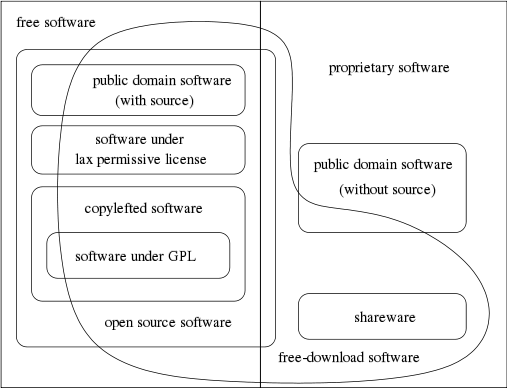
\includegraphics[width=\textwidth]{license-categories}
          		\caption{Taxonomía de Licencias Software}
            \end{center}
        \end{figure}
        
        \paragraph{}
        
        
        \subsection{Licencias Libres y de Código Abierto}
        
			\paragraph{}
            Antes de abordar un tema tan amplio como son las licencias de software libre y de código abierto, puesto que es habitual confundir ambos términos, definiremos estos conceptos para una mejor comprensión del contenido de la sección, ya que se encuentran estrechamente relacionados pero tienen sutiles diferencias que es importante conocer.
            
            \subsubsection{Copyleft}
            \paragraph{}
            El copyleft es una práctica la cual permite la libre distribución de copias o modificaciones de un trabajo u obra, exigiendo que los mismos derechos de copyleft se apliquen a dichas copias o modificaciones. Este termino surge en las comunidades de software libre. Se considera que una licencia software libre es copyleft cuando además de otorgar permisos de uso, copia, modificación y redistribución, contiene una clausula que dispone una licencia similar o compatible a las copias y productos derivados.\cite{Wikipedia:Copyleft}
            
            \subsubsection{Código Abierto}
            \paragraph{}
            Se entiende por código abierto aquel software que se distribuye y desarrolla de forma libre, es decir, se centra en los beneficios prácticos como el acceso al código fuente o la posibilidad de poder modificar dicho código sin restricciones de licencia. Por lo tanto, es software que se puede usar, escribir, modificar y redistribuir gratuitamente.\cite{Wikipedia:CodigoAbierto}
            \paragraph{}
            La idea del código abierto se centra en que al compartir el código fuente el software tiende a ser de mejor calidad que el software propietario. Este software ha de cumplir unos requisitos para que pueda considerarse de este tipo, estos requisitos son:
            \begin{itemize}
            \item \textbf{Libre redistribución:} El software debe poder venderse o regalarse libremente.
            \item \textbf{Código fuente:} El código fuente debe incluirse en la distribución o poder obtenerse libremente.
            \item \textbf{Trabajos derivados:} Las modificaciones sobre el código deben poder redistribuirse libremente.
            \item \textbf{Integridad del código original:} Las licencias pueden requerir que las modificaciones sean redistribuidas como parches y no como un nuevo software.
            \item \textbf{No discriminatorio:} Las licencias no pueden discriminar ninguna persona o grupo social, ni tampoco ningún área de iniciativa como usuarios comerciales.
            \item \textbf{Igualdad:} Deben aplicarse todos los mismos derechos a todo el que reciba el software.
            \item \textbf{Licencia no especifica:} El software no puede licenciarse como parte de una distribución mayor.
            \item \textbf{Licencia no restrictiva:} La licencia no puede obligar a que cualquier otro software que sea distribuido con el software abierto sea también de este tipo.
            \item \textbf{Licencia tecnológicamente neutral:} No debe requerirse la aceptación de la licencia por medio del soporte software.
            \end{itemize}
            
            \subsubsection{Software Libre}
            \paragraph{}
            El software libre se define como el conjunto de software que por elección manifiesta de su autor, puede ser copiado, estudiado, modificado, utilizado con cualquier fin y redistribuido con o sin mejoras o cambios. El nacimiento de este software viene de la mano de Richard Stallman y en 1985 la fundación de software libre (FFS).\cite{Wikipedia:SoftwareLibre}
            
            \paragraph{}
            Para que un software pueda ser considerado "libre" cuando garantiza las siguientes libertades:
            \begin{itemize}
            \item \textbf{Uso:} La libertad de usar el software, con cualquier propósito.
            \item \textbf{Estudio:} La libertad de estudiar cómo funciona el software adaptándolo a las necesidades personales.
            \item \textbf{Distribución:} La libertad de distribuir copias del software.
            \item \textbf{Mejora:} La libertad de mejorar y hacer publicas dichas mejoras, de modo que la comunidad se pueda beneficiar de estas.
            \end{itemize}
            
            \paragraph{}
            Por lo tanto las diferencias entre estos dos conceptos son: El software libre hace gran hincapié en las cuestiones morales y éticas relacionadas con el software, viendo el aspecto técnico como algo secundario. Por otra parte el código abierto establece este aspecto técnico como prioritario, siendo esta su mayor diferencia. Otra diferencia, posiblemente la más importante es el aspecto del comercio. Bajo los estándares de software libre se puede obtener remuneración por conceptos de desarrollo o mantenimiento siempre y cuando se entreguen los códigos fuente, a diferencia del código abierto el cual no obliga a ello. Es decir, todos los derivados del software libre han de ser siempre libres.
            
            \paragraph{}
            Por lo tanto una licencia es básicamente un contrato entre el autor del software y el usuario del mismo en la que se establece una serie de clausulas y términos que el usuario debe cumplir para utilizar dicho software. La definición del concepto de licencia es aquella autorización formal de carácter contractual que el autor del software otorga a un interesado para ejercer derechos de explotación legales.
            
            \paragraph{}
            Sobre un mismo producto software puede haber varias licencias, tantas como acuerdos concretos se establezcan entre el autor del software y el licenciatario. Dentro del software libre existen una gran cantidad de licencias disponibles, algunas de las mas usadas son: AGLP (Affero General Public License), BSD (Berkeley Software Distribution), Apache Licenses, MIT License y GNU GPL (General Public License) la cual es la más utilizada en la actualidad. Las posteriores subsecciones se centraran en los aspectos referentes a estas licencias.\cite{BBVA:Licencias} \cite{UCLM:Licencias}
            
            \subsubsection{Licencias GNU GPL}
            	\paragraph{}
                Esta licencia es la más utilizada a nivel global en el campo del software, con la licenciación de software a través de esta licencia se garantiza a los usuarios finales la libertad de usar, estudiar, redistribuir copias o modificar dicho software. Aproximadamente el 60\% del software esta licenciado bajo GNU GPL.
                
                \paragraph{}
                La GPL puede ser utilizada por cualquiera, ya que su finalidad es declarar que el software cubierto por esta licencia este protegido de intentos de apropiación que restrinjan las libertades a los usuarios finales. El autor de dicho software mantiene los derechos de copyright. Bajo esta idea, la GPL garantiza a los usuarios que este software cumple con las libertades y derechos del software libre, ya sea para su uso modificación o bien para su ampliación. Cualquier software derivado de este que sea distribuido debe ser licenciado bajo GPL, protegiendo de esta forma la filosofía del software libre.
                
                \paragraph{}
                El código licenciado bajo GNU GPL no podrá ser entrelazado ni mezclado con otro código con una licencia la cual incluya requisitos no contemplados por la GPL. En caso de mezclar con código no licenciado el producto resultante deberá licenciarse bajo GNU GPL.
                
		\subsubsection{Licencias AGLP}
        	\paragraph{}
             AGPL o Affero GPL es una licencia de copyleft derivada de GNU GPL utilizada ampliamente sobre software el cual se ejecuta sobre servidores de red. Esta licencia garantiza la cooperación de la comunidad a la hora de mantener mejorar o ampliar este software. Básicamente es una licencia GNU GPL con una nueva cláusula la cual añade la obligación de que el software que corra sobre una red debe ser distribuido a todos los usuarios de dicha red.
             
        \subsubsection{Licencia BSD}
        	\paragraph{}
            La licencia BSD es una licencia software la cual fue aplicada inicialmente a los sistemas BSD(Berkley Software Distribution), un tipo de sistemas Unix. Es una licencia software libre permisiva al igual que OpenSSL y MIT License. Lo que entra en conflicto con las características del copyleft ya que defiende el ''compartir-igual''.
            
            \paragraph{}
            Esta licencia es la más cercana al dominio público, debido a las pocas restricciones que impone a los usuarios finales de los productos software licenciados bajo ella. La licencia BSD permite la reutilización de código fuente en productos de software no libre, incluyendo una cláusula la cual determina la aprobación y reconocimiento del autor para la reutilización del código en software no libre.
             
  		\subsubsection{Licencia MIT}
        	\paragraph{}
             La licencia MIT (Massachusetts Institute of Technology) es una licencia de software libre permisiva, lo que implica que impone muy pocas restricciones a la hora de las reutilizaciones lo que le proporciona una gran capacidad de compatibilidad de licencias, todo lo contrario que GNU GPL y sus derivados. Código licenciado con MIT puede integrarse con código licenciado con GPL. De forma contraria, el código GPL no puede integrarse con código MIT debido a las restricciones que impone GPL.
             
             \paragraph{}
              La licencia MIT permite la reutilización de software en productos de software propietario, a diferencia de la BSD no incluye la clausula de aprobación. Es una de las más populares en el mundo del software, en 2015 gracias a un acuerdo con Black Duck Software y GitHub llego a ser la más utilizada, por encima incluso de las licencias GPL. En cuanto a efectos de su uso es muy parecida a la licencia BSD.
              
     	\subsubsection{Licencia Apache}
        	\paragraph{}
        	Como cualquier otra licencia software libre, la licencia Apache permite al usuario usar, modificar, copiar y redistribuir el software. La licencia Apache es permisiva, ya que no obliga a que los trabajos derivados del software se distribuyan bajo la misma licencia, ni que tengan que ser distribuidas como software libre.
            
            \paragraph{}
            La licencia Apache sólo exige que se mantenga un aviso que informe a los receptores que en la distribución se ha usado código con la licencia Apache. En cada distribución de los productos se debe añadir una copia de la licencia, así como un archivo de texto en el cual se incluyan los avisos obligatorios del software de esta distribución. El contenido de este archivo no modifica la licencia, ya que son solo para fines informativos. 
                
            
        \subsection{Licencias Propietarias}

			\paragraph{}
            Las licencias de software propietarias abarcan un amplio rango de posibilidades en cuanto a los permisos de uso, modificación o distribución del software, pero todas ellas se diferencian del resto debido a la prohibición de alguna de estas posibilidades. Por contra, existen algunos casos en que para poder optar a alguna de estas posibilidades es necesario obtener permiso expreso del titular de dicho software.
            \paragraph{}
            A continuación se describen más en detalle las características de estos permisos:
            \begin{itemize}
            	\item \textbf{Permiso de Uso}: En el caso de las licencias propietarias en cuanto al uso del sistema, se permite desde requerir la autorización del creador (en la mayoría de casos pagando por ello) hasta permitir que el usuario acceda sin esta. Sin embargo, en la mayoría de casos en que esto ocurre se suele recurrir a otras maneras de financiación como la publicidad.

            	\item \textbf{Permiso de Modificación}: En este tipo de licencias por lo general no está permitido el derecho de modificación del sistema sin la autorización expresa por parte de su creador. Además, en la mayoría de casos el código fuente no está disponible públicamente para que cualquiera lo pueda visualizar.

            	\item \textbf{Permiso de Distribución}: Las licencias propietarias  generalmente suelen estar caracterizadas (aunque existen excepciones) por su orientación hacia los beneficios económicos. El modo en que se conseguía esto en el pasado era exigir un pago por obtener una copia del sistema. Sin embargo, estas estrategias se han ido orientando hacia el uso de claves o licencias de acceso, por lo cual, en la actualidad muchos sistemas software con licencias propietarias se pueden distribuir sin restricciones (siempre y cuando se cumplan los requisitos fijados de uso y modificación). 

            \end{itemize}
            
            \paragraph{}
			Tal y como se puede comprobar, la perspectiva que se ofrece a partir de este tipo de licencias se contrapone con el de las libres y de código abierto.
			
            \subsubsection{Derecho de Autor}
            
            	\paragraph{}
            	Este conjunto de ideas no es algo inherente al software únicamente, sino que se aplica a muchas otras ramas del conocimiento y las artes, que se pueden englobar dentro de un concepto más general denominado \emph{derecho de autor}. Por tanto, a continuación se describe más en detalle dicho término.
            
           		\paragraph{}
				El \textbf{derecho de autor} constituye uno de los principales derechos de propiedad intelectual, cuyo objetivo es dar solución a una serie de conflictos de intereses, que nacen entre los autores de las creaciones intelectuales, los editores y demás intermediarios que las distribuyen con el público que las consume. Estos derechos se reconocen en la \emph{Declaración Universal de Derechos Humanos}. Por lo general, tienen una duración determinada y una vez superada su fecha de espiración se añaden al dominio público (engloba el patrimonio intelectual que está libre de toda exclusividad en su acceso y utilización).

			\subsubsection{Software Privativo}

				\paragraph{}
                Muchos de los defensores de la comunidad del Software Libre están en contra del uso del término \emph{propietario} para referirse a este tipo de licenciatura. El motivo que exponen para defender esto es que el término Software Propietario ha sido introducido por las grandes empresas del sector como campaña para tratar de desacreditar el Software Libre, alegando que este no tiene garantías legales acerca de su corrección. 
                
                \paragraph{}
				Por este motivo,  Richard Stallman comenzó a introducir en el año 2003 el término \emph{Software Privativo}, ya que según él, es más afín a las ideas que los sistemas bajo este tipo de licencias utilizan. 

                \paragraph{}
				También ha cobrado fuerza el término \emph{software de código cerrado}, cuya definición es el antónimo de software de código abierto, es decir, aquel que no permite la visualización de su código fuente y por tanto, solo ofrece los ejecutables del sistema. Dentro de 
   
			\subsubsection{Freeware}
               	
               	\paragraph{}
                La palabra \textbf{freeware} no posee una definición estricta y claramente aceptada. Se usa generalmente para definir el software que permite su redistribución, pero por contra, no permite ser modificado, es decir, su código fuente no está disponible. Por tanto, este no se puede englobar dentro de la categoría de software libre. Desde la comunidad de Software Libre se desaconseja el uso de este término para referirse a esa categoría por los motivos expuestos previamente.


			\subsubsection{Shareware}
                
                \paragraph{}
                El término \textbf{shareware} se refiere al software que permite su redistribución, pero por contra, para poder utilizarlo se necesita algún tipo de licencia o clave que el creador suministra a cambio de un pago. El motivo por el cuál este software no se puede clasificar dentro del libre tiene dos razones principales:
                
                \begin{itemize}
	                \item En la mayoría de los casos el código fuente no está disponible públicamente, por lo cual, se restringe su permiso de modificación.
                    \item Su uso requiere el pago por una licencia de uso, aún en los casos en que no existan fines lucrativos.
                \end{itemize}


			\subsubsection{Software Privado}
				
                \paragraph{}
                El término \textbf{Software Privado} se refiere a aquel software cuyo creador no publica, sino que él mismo mantiene y utiliza. Por lo tanto no está disponible ni como código fuente ni como binarios. Esta idea tiene sentido en casos en que un determinado usuario (generalmente empresa) demanda un sistema software para un caso concreto y personalizado que probablemente no será extrapolable a otras situaciones o contextos. La mayoría de los defensores del Software Libre no están en contra de esta idea debido a que entienden que este tipo de software no aporta demasiado a la comunidad.
                
         	\subsubsection{Licencias propietarias más extendidas}
                
                \paragraph{}
                El software propietario incluye tanto variantes libres como no libres dentro de su distribución, es decir, se considera fuente mixta. La mayoría del software propietario basado en UNIX normalmente incluye componentes de código abierto, como Sendmail, X Window System y DHCP, además de las utilidades del sistema cerradas y propietarias.

                \paragraph{}
				Las empresas no siempre cobran por su software propietario, aunque bloquean el acceso al código fuente e imponen restricciones sobre su uso. Internet Explorer es un ejemplo de software propietario que está disponible de forma gratuita, mientras que la mayoría de los otros productos ofrecidos por Microsoft, incluyendo su familia de sistemas operativos Windows y Microsoft Office, requieren una tarifa para adquirir una licencia. Oracle, Macromedia, Adobe e IBM son otras empresas además de Microsoft que casi exclusivamente producen software propietario. Las restricciones con respecto al uso del software se delinean típicamente en el acuerdo de licencia del usuario final y los términos del servicio.

                \paragraph{}
				Desde 2014, los analistas de la industria opinan que el uso de software propietario está en declive debido a la creciente disponibilidad de software de código abierto que potencialmente podría dominar el mercado, girando en torno a los sistemas operativos y otras aplicaciones en el futuro.
                
                \paragraph{}
                \textbf{CreativeCommons} es una de las varias licencias públicas de derechos de autor que permiten la distribución gratuita de una obra pero a la vez con derechos de autor. Una licencia CC se utiliza cuando un autor quiere dar a la gente el derecho de compartir, utilizar y construir sobre una su obra.
                
		\subsection{Uso Comercial}

			\paragraph{}
			Otro de los conceptos que involucra el uso de licencias propietarias es el \textbf{uso comercial}. Lo que se pretende con esto es compatibilizar la idea software libre en los casos en que el usuario del software no vaya a obtener beneficios económicos. 
      		\paragraph{}
			Su uso se ha extendido mucho en los últimos años. La causa de su extensión se ha debido a que cada vez más empresas de desarrollo de software empresarial ofrecen sus productos gratuitamente para uso personal. Lo que pretenden con esta estrategia es que el usuario pueda probar la herramienta y familiarizarse con ella, lo que facilita que este esté dispuesto a pagar por ella para poder utilizarla en su trabajo.
                	




    \section{Recomendaciones sobre el uso de licencias}
		
        \paragraph{}
        Una vez seleccionado el tipo de licencia que se va a utilizar, se debe tener en cuenta las responsabilidades que el usuario final tiene con esa licencia, sobre todo en el caso de las licencias propietarias. Este tipo de licencias son posiblemente las más reguladas y controladas por la legislación de los países y el fraude cometido con respecto a ellas puede constituir delitos graves contra la propiedad intelectual con multas muy significativas. En esta sección se va a desglosar el cómo utilizar correctamente las licencias y las consecuencias que puede acarrear el mal uso de las mismas.
        
        \subsection{Recomendaciones sobre el uso de licencias de software libre y de código abierto}
        \paragraph{}
        Las empresas de software libre no destinan recursos en proteger y beneficiarse de los derechos de explotación sobre su software, por lo que aseguran a los usuarios  una libertad total que les permite:
        \begin{itemize}
        \item Uso del software
        \item Modificación del software
        \item Redistribución del software con o sin modificaciones
		\item Lucrarse de la redistribución del software, proporcionando un beneficio económico
        \end{itemize}
        \paragraph{}
        A pesar de todo existen dos condiciones esenciales, aunque no están apenas regidas o aseguradas por ninguna ley pero que los usuarios de software libre deben cumplir:
		\begin{itemize}
		\item Reconocer y respetar al autor del software
		\item Asegurar el respeto a las libertades ya mencionadas en esta sección por parte del resto de los usuarios de dicho software
		\end{itemize}

		\paragraph{}
        Este tipo de licencias están respaldadas por la ley gracias al concepto \textit{copyleft} ideado para regularizar la concepción de libertad de expresión asociada al software libre y determinar los límites en los que se encuadran las operaciones de distribución, producción y utilización del software libre, como ya se ha mencionado con anterioridad en este documento.
        
        \subsection{Recomendaciones sobre el uso de licencias de software propietario}
        \paragraph{}
        Las empresas que usan licencias de software propietario deben tener en cuenta que no tienen la misma libertad de uso que las de software libre ya mencionadas en la sección anterior. Estas empresas deben conocer una serie de características y buenas prácticas a la hora de utilizar este tipo de licencias.
        \begin{itemize}
        \item No se puede realizar ningún tipo de modificación al código fuente del software
        \item No se puede distribuir sin el permiso del propietario
        \item La licencia propietaria puede incluir otras restricciones de uso marcadas por el propietario
        \item Imposibilidad de copia del software
        \item En algunos casos la empresa deberá realizar cursos para aprender a utilizar este tipo de software
        \item Se debe tener en cuenta el costo de la licencia a la hora de implementar este tipo de software en la empresa
        \end{itemize}
        Hay que tener en cuenta que este tipo de licencias están respaldadas por acuerdos legales y que su incumplimiento puede conllevar un delito, en el caso de copia y redistribución del software propietario se incide en un delito contra la propiedad intelectual. Las instituciones encargadas de la regulación del buen uso de este tipo de software pueden realizar auditorías para comprobar que las licencias se estén usando correctamente y no haya ningún uso ilícito del software.
        
        \subsection{Software libre vs Software propietario}
        \paragraph{}
        Como se ha mencionado en las secciones anteriores, tanto el software libre como el software propietario tienen sus ventajas y sus desventajas, y se diferencian mayoritariamente en el poder por parte del usuario de acceder al código fuente, modificar el software o incluso redistribuirlo. En el siguiente gráfico se pueden observar las mayores diferencias entre uno y otro.
        
        \begin{figure}[htb]
            \centering
            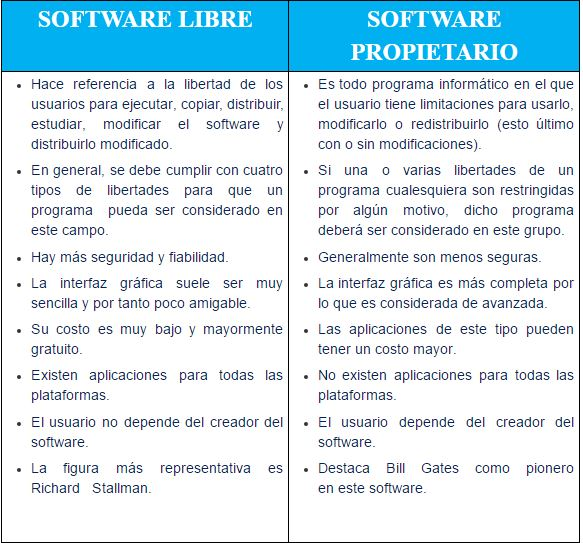
\includegraphics[width=0.6 \textwidth]{Captura-PyS.JPG}
            \caption{Software libre vs Software propietario}\label{vs}
        \end{figure}
        
        
        \paragraph{}
        La creencia más extendida para diferenciar el software libre y el software propietario es el que el software libre es gratuito y el software propietario tiene un coste económico. Como se ha mencionado anteriormente en este documento eso no es cierto ya que las licencias freeware no tienen un coste económico pero siguen perteneciendo a la clasificación de software propietario.
        
        \paragraph{}
        Principalmente la diferencia entre software libre y software propietario se atribuye a una serie de libertades, que si se garantizan todas ellas el software será posible clasificarlo como libre, y en caso contrario como propietario.
        \begin{itemize}
        \item La libertad de usar el programa, con cualquier propósito.
        \item La libertad de estudiar cómo funciona el programa, y adaptarlo a las necesidades que se estimen oportunas.
        \item La libertad de distribuir copias.
        \item La libertad de mejorar el programa y hacer públicas las mejoras al resto de la comunidad, para que ésta se beneficie de ellas.
        \end{itemize}
        \paragraph{}
        Una vez clasificado el tipo de software que se tiene la regulación es parecida. En España la ley de propiedad intelectual es la encargada de regular en su \textit{título VII}\cite{Ley:tit7} la protección de los derechos de autor de los creadores de los programas de ordenador. En dicho artículo, la ley prohibirá a todo aquel que no sea el titular de estos derechos la reproducción total o parcial, o cualquier transformación o distribución del producto, siempre y cuando la licencia de este software impida lo ya mencionado anteriormente.
        
        \paragraph{}
        Por otra parte el software libre cuenta con sus propias medidas de protección. Organismos de referencia como la \textit{Free Software Foundation} mantienen en sus webs oficiales listados de las licencias de software libre que aprueban. Estos instrumentos jurídicos regulan el funcionamiento de los mecanismos de redistribución, creación y copia de los mismos.
        
        \paragraph{}
        Otra de las diferencias entre estos dos tipos de licencia es la concepción del software, mientras que los creadores de  software propietario o privativo es concebido como un producto, el software libre es concebido como un servicio. Esta clasificación refleja que el software privativo es un producto por el que se pretende obtener una remuneración y el software libre es tratado como un servicio que se ofrece a la comunidad.
        
    \newpage
    
    \section{Conclusiones}
    
    	\paragraph{}
        Como se ha visto a lo largo de este trabajo, las licencias software son un tema de estudio muy amplio y variado debido a la gran cantidad de tipos que existen. Toda esta variedad de formas de proteger el software supone el estudio meticuloso por parte de los desarrolladores.

        \paragraph{}
        Las diferencias entre la gran cantidad de licencias disponibles es, en muchas ocasiones, muy sutil. Esto implica que se deba tratar con cautela su estudio para imponer adecuadamente la protección legal deseada. Sin una buena elección, el producto quedará completamente desprotegido ante la voluntad del propietario.
        
        \paragraph{}
        En definitiva, se puede concluir en que las licencias software constituyen una herramienta necesaria para la puesta en producción de un sistema software y que sin ellas, no existiría un método para proteger legalmente el trabajo de los ingenieros de software.
        
        
       \newpage 
%----------------------------------------------------------------------------------------
%	Bibliographic references
%----------------------------------------------------------------------------------------
	\begin{thebibliography}{9}
    
        \bibitem{wikipedia:propietary}
        Wikipedia: Propietary Software \url{https://en.wikipedia.org/wiki/Proprietary_software}
        
        \bibitem{gnu:categories}
        GNU: Categories of free and nonfree software \url{https://www.gnu.org/philosophy/categories.en.html}
        
        \bibitem{monografias: s.libre y propietario}
        Monografias: Uso de software libre y propietario
\url{http://www.monografias.com/trabajos89/sotware-libre-y-propietario/sotware-libre-y-propietario.shtml#softwarepa}

		 \bibitem{FFS:Licencias}
        FFS: Definición y características de las licencias libres por la FFS\url{https://opensource.org/licenses/GPL-3}
        
        \bibitem{Wikipedia:Copyleft}
        Wikipedia: Información sobre el copyleft\url{https://es.wikipedia.org/wiki/Copyleft}
        
        \bibitem{UCLM:Licencias}
        UCLM: Documento sobre licencias libres por la Universidad de Castilla la Mancha\url{http://biblioteca.uclm.es/Archivos/Investigacion/Software\_libre.pdf}
        
        \bibitem{B: software libre vs software propietario}
        Blog: Gráfico que enfrenta el software libre con el software propietario
  \url{http://sis19upt.blogspot.com.es/2012/03/software-libre-y-software-propietario.html}
  
  		\bibitem{COBDC: libre vs propietario}
        COBDC: Software libre vs software propietario       \url{http://www.cobdc.net/programarilliure/software-libre-software-propietario-legislacion-modelos-negocio/}
        
        \bibitem{Ley:tit7}
        Ley propiedad intelectual: título VII
\url{http://noticias.juridicas.com/base_datos/Admin/rdleg1-1996.l1t7.html#l1t7}
        
        \bibitem{Laurent:Book}
        Andrew M. St. Laurent: Understanding Open Source and Free Software Licensing
\url{http://www.oreilly.com/openbook/osfreesoft}

        
        \bibitem{Reference:question}
        Reference: What are some examples of proprietary software?
\url{https://www.reference.com/technology/examples-proprietary-software-5ce70357b540aeed

}

		\bibitem{Merchadlinux:SoftwareLicenses}
        Merchandlinux: Licencias para el software de código abierto.
\url{https://merchandlinux.wordpress.com/2009/04/02/licencias-para-el-software-de-codigo-abierto-open-source/}

		\bibitem{Wikipedia:SoftwareLibre}
        Wikipedia: Software libre
   		\url{https://es.wikipedia.org/wiki/Software_libre}
        
        \bibitem{BBVA:Licencias}
        BBVA: 5 licencias de software libre que debes conocer
        \url{https://bbvaopen4u.com/es/actualidad/las-5-licencias-de-software-libre-mas-importantes-que-todo-desarrollador-debe-conocer}
        
        \bibitem{Wikipedia:CodigoAbierto}
        Wikipedia: Código abierto
        \url{https://es.wikipedia.org/wiki/C%C3%B3digo\_abierto}




        
	\end{thebibliography}
  
		
\end{document}


